% -------------------------------------------------------------------------------------------------
%      MDSG Latex Framework
%      ============================================================================================
%      File:                  introduction-[UTF8,ISO8859-1].tex
%      Author(s):             Michael Duerr
%      Version:               1
%      Creation Date:         30. Mai 2010
%      Creation Date:         30. Mai 2010
%
%      Notes:                 - Example chapter
% -------------------------------------------------------------------------------------------------
%
\chapter{Approach}\label{sec:Concept}
- What is your plan? \\
- How do you proof that it worked? -> Metric and Experiments


\section{Coloring Environment}\label{env}
\marginpar{origin and intro}
% Introduce Gridworld, Agent actions, goal etc.
A RL environment is a versatile and unbiased instance, that can can be used to visualize agent behavior and environmental changes.
% Although a human visualization is optional, agents need to have some sort of understanding what state they are acting in. 
In figure \ref{fig:env}, the environment used in this work is presented. It originated from an openAI project called ``Minimalistic Gridworld Environment'' \cite{chwi18}, which is designed for one agent whose main goal is to solve labyrinth puzzles. For the purpose of this research however, the environment is changed heavily, becoming the ``Coloring Environment''. Multiple agents can act in the new instance to try and achieve a new goal - to color all walkable cells.

\begin{figure}[hpbt]
    \centering
    %%----start of first subfigure----
    \subfloat[Human visualization of the coloring environment. A dot represents one agent. Cells change their color when agents move on them.]{
        \label{fig:env} %% label for first subfigure
        \includegraphics[width=0.35\linewidth]{pictures/Gridworld}}
    \hspace{0.01\textwidth}
    %%----start of second subfigure----
    \subfloat[Simplified agent observation of the current environment state. The number 1 represents a colored cell.]{
        \label{fig:bin_env} %% label for second subfigure
        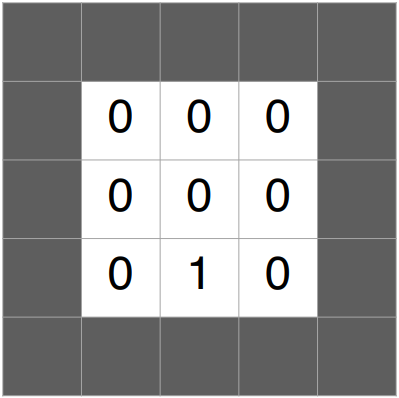
\includegraphics[width=0.35\linewidth]{pictures/binary_gridworld}}
    \caption[Coloring Environment]{Representations of the coloring environment}
    \label{fig:multipic_env} %% label for entire figure
\end{figure}

\marginpar{cell objects}
Figure \ref{fig:bin_env} shows a simplified environment observation an agent processes each time step. Every environment cell holds information about the object it represents, being either Walls, Floors or Agents. Furthermore, each object class contains information about its current color, whether it is accessible for an agent and, in case of a floor tile, if it is colored. 

\subsection{Compositions}
\marginpar{compositions}
When multiple agents are placed in the coloring environment together, there are several ways how they will behave towards each other. Depending on the setting, even the environment distinguishes how certain actions affect the state. Per default agents will try to work together, to reach the environment goal. Alternatively, they could work independently or even compete with each other.

\marginpar{floor coloration}
Floor cells manage the coloration state in binary form, as displayed in \ref{fig:bin_env}, with a 1 signalizing that the cell is colored. The environment reacts to agent movements by coloring the cells they visit. Agents successfully solve the environment once all fields are colored. Otherwise, agents loose by using up a limited amount of steps.

\marginpar{bit switching}
If a cell is already in coloration state 1 and an agent walks over it again the bit is switched, and the cell is reset to 0, removing the color. Besides moving up, down, left and right an agent can also execute the action wait, to stay in place.

\marginpar{cooperative multiagents}
Each agent has a different random color. Cells adopt the color of the agent that walks over it. The primary focus in cooperative agent compositions however, is only the binary state. All agents always receive the same reward, regardless of the coloration. An extreme example would be one agent that color the whole grid on its own, and all other agents would profit from the same high reward. 

In a DR setting however, agents are able to estimate their contribution, in order to improve their actions. This implementation executes the default action wait to find $G(z_{-i})$, see equation \eqref{eq:dr}. By choosing wait as the default action, agents can learn what the environment outcome and general coloration percentage would be if they had not participated in the current step. It is important to not here, that DR settings are always an extension of the cooperation mode and are never used together with market additions.

\marginpar{mixed-motive multiagents}
% The opposite is the case in competitive scenarios. 
In mixed-motive settings the colors are of importance. Agents only gain rewards based on their individual contributions. Thus, the rewards are generated by looking up each percentage a color is present and assigning that value to the same colored agent as reward. For example if the red agent 1 colored 60\% of the grid red the reward for that agent would be 0.60. All other agents receive their individual color percentages.

\marginpar{competitive multiagents}
In a fully competitive mixed-motive scenario the reward calculations stay the same, only disabling the bit switching for opponent colors. Therefore, agents can directly capture already colored cells when they walk over them. However, if the captured cell contains the same color as the agent the cell is reset instead. Hence, taking over the cells of the opponents is beneficial, since it increases the color presence of the own color, leading to a higher reward.

\marginpar{comparison multiagents}
In comparison, the basic mixed-motive composition shows no advantages resetting colored cells. This implementation punishes the resetting of cells with a small negative reward. Since the cell is not captured, the agent won't receive more reward. Hence, it is not likely that the agents work against each other yielding an agent composition with neutral or independent behavior.

\subsection{Observation}
\marginpar{what the agent sees}
The observations agents receive from the environment are always generated from their individual point of view, with them in the center. The observation only contains a restricted area around them, making the environment a partially observable MDP. In large environments this feature increases the difficulty.
%but at the same time reflects the reality. 
An example for an observation of an agent is shown in \ref{fig:agent_obs}. This observation depicts the internal state of the environment visualization of image \ref{fig:env}.

\begin{figure}[hpbt]
    \centering
    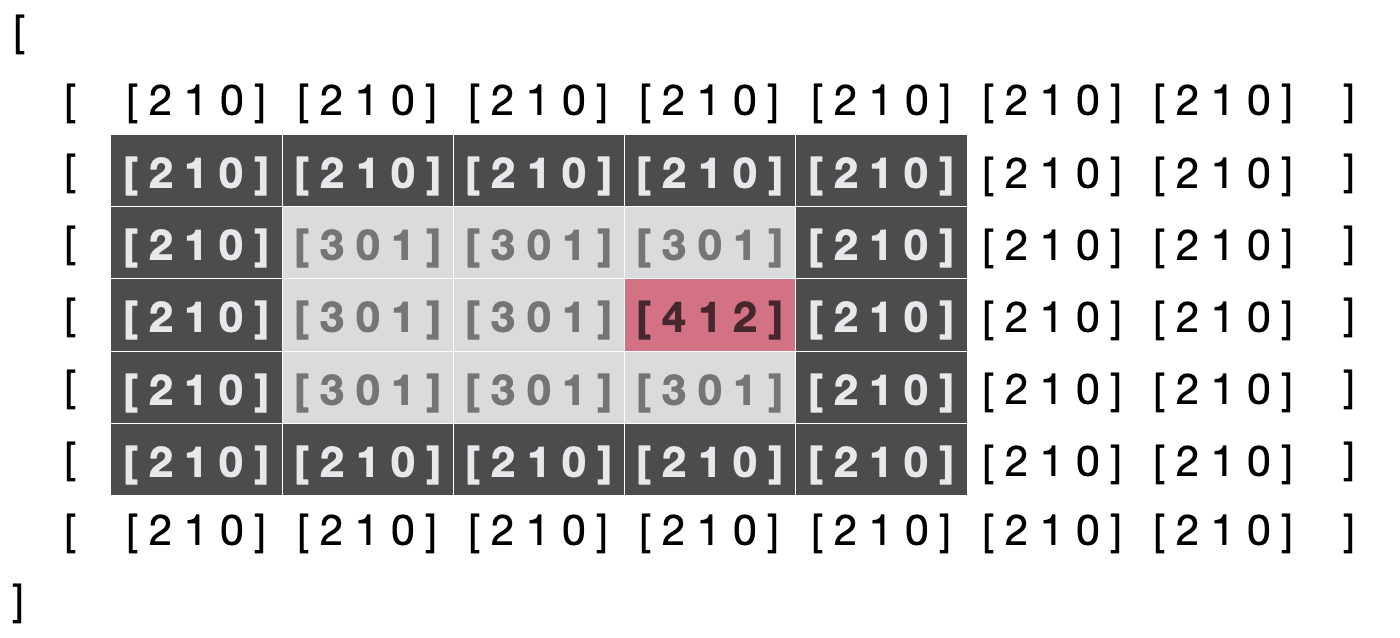
\includegraphics[width=0.8\textwidth]{pictures/agent_observation}\\
    \caption[Agent Observation]{The internal agent observation}\label{fig:agent_obs}
\end{figure}

\marginpar{description and dimensions}
Per default the agent has a view size of a seven by seven grid, represented in a three-dimensional array, similar to a picture with RGB information. Here, all highlighted entries are part of the grid that is shown in Figure \ref{fig:env} and the red array shows the agent. The first dimension of the observation array contains the whole internal observation of an agent. The second array dimension represents the environment grid. Since the view size of the agent exceeds the dimension of the 5x5 visual grid, the additional rows and columns are filled with placeholders, in this case walls. All highlighted row entries can be mapped to the columns of \ref{fig:env}, starting from the top left of the visualization. The last dimension contains cell information, which is always composed of three elements. 

% This also reduces the complexity of checking for a fully colored grid by just looking at all coloration states, regardless of the object type.

\marginpar{cell encoding colors}
The first cell element defines the object type with 1 being just an empty cell, 2 shows a wall, 3 a floor tile and 4 an agent. The second element stores the coloration status, showing whether a cell is colored, with zero signalizing an uncolored cell. Since agents can not walk onto walls, represented as $[\;2\;1\;0\;]$, that object type always has a coloration state of 1. The third cell encoding describes the color of a cell. To better distinguish the types in the visual representation, walls are 0 for the color black and floors are initially white with encoding 1. Each agent is assigned a number from 2 upwards which in turn stands for a randomly generated RGB color. The Floor color encoding is overwritten with the agents color code when the cell is captured. For example, should the agent move to the left, the cell of the previous position is now a colored Floor cell $[\;3\;1\;2\;]$. The new position of the agent is now in row three and column four with cell encoding $[\;4\;1\;2\;]$.

\section{Reward Calculations}\label{reward_calculations}
\marginpar{activation line}
The allocation of rewards is closely related to the composition of the agents, which can be specified by the user in training or visualization runs. In addition, the environment shape can be set, a number of agents placed and more. A basic example command for a training run is shown in listing \ref{lst:command}.

\begin{lstlisting}[float=htp,caption=Exemplary command to execute training with three agents in a coloring environment using PPO as algorithm,label=lst:command,language=bash, numbers=left, numberstyle=\tiny, numbersep=8pt, escapeinside={//@}{@//},xleftmargin=3ex,xrightmargin=1ex]
$ python -m Coloring.scripts.train
    --algo ppo
    --model ppo-training
    --env Empty-Grid-v0 
    --grid-size 7
    --agents 3 
    --max-steps 350
    --setting mixed-motive
\end{lstlisting}

\marginpar{command algo and model}
The \verb|--algo| parameter can be either ``ppo'' or ``dqn'' to choose a learning algorithm. This argument is the only required setting for training. All other configurations, including those not listed in \ref{lst:command}, have default values and are listed in Appendix \ref{ax:training_params}.
%  discussed in the sections \ref{learning_process} and \ref{market_settings}. An overview of all training parameters and their default values is listed in .
With \verb|--model| the destination path is defined, in which all logs, recordings and status updates are stored. Line 4 and 5 configures the environment. Alternatively to the empty grid option of \verb|--env|, as shown in figure \ref{fig:env}, four homogeneous rooms can be generated with ``FourRooms-Grid-v0'' to increase the difficulty. The rooms are always of the same size and each room is accessible to all adjoining neighbors by one wall opening, which is random and changes in each episode. The overall size of the grid is set in Line 5. However, all grids in every layout option have outer walls that narrow the area in which agents can move. Hence, in a grid of size 7 the agents can only move in a 5 by 5 field, due to the surrounding walls.

\marginpar{settings}
The amount of agents that act in the environment is set through the argument \verb|--agents| and the maximum quantity of steps they can execute is defined with \verb|--max-steps|. To gain the highest reward, the agents need to color the whole field before they run out of steps. Lastly, the argument \verb|--setting| specifies the composition of the agents. If no setting is set the agents work cooperatively. In the example of \ref{lst:command} the setting ``mixed-motive'' is chosen. The last two options here are ``mixed-motive-competitive'' and ``difference-reward''. % and ``percentage''.

\marginpar{environment reward}
Regardless of the composition, agents initially generate separate rewards in each step based on their individual environment change. For instance, agents that color a field produce a positive reward of 0.1, whereas agents that reset a field contribute a penalty of negative 0.1. Agents that just wait generate a reward of 0. The only exception is the setting ``mixed-motive-competitive'', since agents can capture opponent cells. If that is the case they get a positive reward of 0.1 otherwise the rules stay the same. 

Rewards are always written into a list, which is initially returned by the environment, see algorithm \ref{algo:step_reward}, line 1. The position in the list indicates the accountable agent, i.e. a reward list of $[0.1, 0, \cdots ]$ shows that agent 0 is responsible for a reward of 0.1 and so forth. In algorithm \ref{algo:step_reward} the adaptation process of the initial environment rewards during each step is summarized. This process is executed in an environment wrapper, as link between learning or visualization function and the environment itself. The step function of the wrapper takes the training arguments into account, which leads to the four conditions below.

\begin{algorithm}[H]
    \DontPrintSemicolon
    observations, rewards, done, info = environment.step(actions)\;
    \;
    \uIf{difference reward setting} {
        rewards = calculate difference reward for each agent
    }
    \ElseIf{cooperative setting}{
        rewards = calculate one cooperative reward
    }
    \;
    \If{market specified}{
        rewards = execute market actions and return transaction rewards\;
    }
    \;
    \If{done}{
        rewards = calculate final rewards
    }
    \;
    \textbf{return} observations, rewards, done, info\;
    \caption{Reward calculation each step}\label{algo:step_reward}
\end{algorithm}

\marginpar{dr rewards}
The first condition checks for a ``difference-reward'' setting. In this case, the agents work in cooperation but try to solve the CAP by calculating the DR, see function \eqref{eq:dr}. To achieve that, the current reward content is summed up, to summarize the overall current reward. As a result the variable $G(z)$ of the DR equation is now set to the summed value. To find the subtrahend of the equation, the agents are iterated, and their individual calculations take place. Here, the environment rewards are added up again, but this time the reward of the current agent is set to zero. This sum is the value of $G(z_{-i})$ for agent i. The function \eqref{eq:dr} is now applied for each agent and the initial reward list is updated with the individual DRs. 

\marginpar{sum clipping}
The last step of the DR reward update is checking, whether any value exceeds an upper or lower bound. If that is the case then the individual reward is set to the corresponding limit. Otherwise, the current value stays as is. The upper and lower bounds are necessary, due to more participating agents possibly leading to a really big or very small sum. For example, very large sums without bounds could in turn decrease the importance of the final reward for reaching the environment goal. The other extreme are high negative sums demotivating agents to move.

\marginpar{coop}
If the setting is set to the standard cooperation, the reward needs to be changed to a new homogeneous value for each agent, since they share the outcome. Again, the sum of the initial environment reward is calculated and reassigned to each agent position in the rewards array. The reward values must be clipped again in the same procedure as for the DR values. Here however, all rewards of the array are changed to the same clipped value, should the bounds be exceeded. Settings that contain ``mixed-motive'' skip all previous reward updates, since in this case each agent keeps their individual value.

\marginpar{market actions}
As third condition the market argument is checked for a SM or AM. In this case the market transactions changes the rewards. Details of the market process are discussed in Section \ref{market_settings}. One thing to note here is that agents can execute market transactions in each step. For example, they can spend their current reward on actions or shares that are for sale or receive the purchase price from buyers, which in turn modifies the rewards.

\marginpar{done}
The last condition depends on the done flag which signalizes the end of an episode. The environment sets done to true, once either the goal is reached or the maximum step amount is executed. In this case the final reward calculations are applied, see algorithm \ref{algo:final_reward}. The result of those calculations is the final update of the reward variable.

\begin{algorithm}[H]
    \DontPrintSemicolon
    \eIf{mixed setting}{
        \For(){each agent}{
            rewards[agent] += agent color percentage on the grid
        }
    }{// cooperative setting \;
        rewards += overall coloration percentage of the Grid
        
        \If {difference reward setting} {
            rewards = calculate difference rewards
        }
    }
    \;
    \If{market specified}{
        rewards = final market adjustments executed on rewards
    }
    \;
    \textbf{return} rewards\;
    \caption{Final reward calculation}\label{algo:final_reward}
\end{algorithm}

\marginpar{done calculations}
During the final reward calculations, see algorithm \ref{algo:final_reward}, the different agent compositions are checked again. In a mixed setting each agents' grid coloration percentage, based on their color presence, is added to the individual reward. Otherwise, the general grid coloration, regardless of the colors, is looked up and added to each reward value. 

Additionally, the presence of a DR setting needs to be checked here. For the final DR calculations the environment supplies information in the \verb|info| variable. Namely, what the general coloration percentage of the environment would be for each agent, if this agent had executed action wait. Those percentages are subtracted from the cooperative coloration percentage to generate the DRs. Finally, the last market calculations are taken into account, see chapter \ref{market_settings} for details.

\section{Learning Process}\label{learning_process}
% \subsection{Base Class}
\marginpar{Independent learning}
In order to compare different settings and agent compositions easily, each agent manages its own learning improvement, observation and action selection. Therefore, all calculations and estimations are executed independently, for instance policy updates and value estimations. They also set up their own neural networks and optimizers and update them only with their own values. However, observations still connect the agent experiences, by including the positions of all agents on the grid and reacting to their joint actions in each step.

\marginpar{process structure}
Depending on the learning algorithm the corresponding class is instantiated by the training script, as shown in Figure \ref{fig:training}. The PPO and DQN classes both extend a base class that provides some abstract methods and a multiprocessing operation to execute actions on several environments at once. The base class returns data, allowing the training script to create recordings and log files to enable evaluation.

\begin{figure}[hpbt]
    \centering
    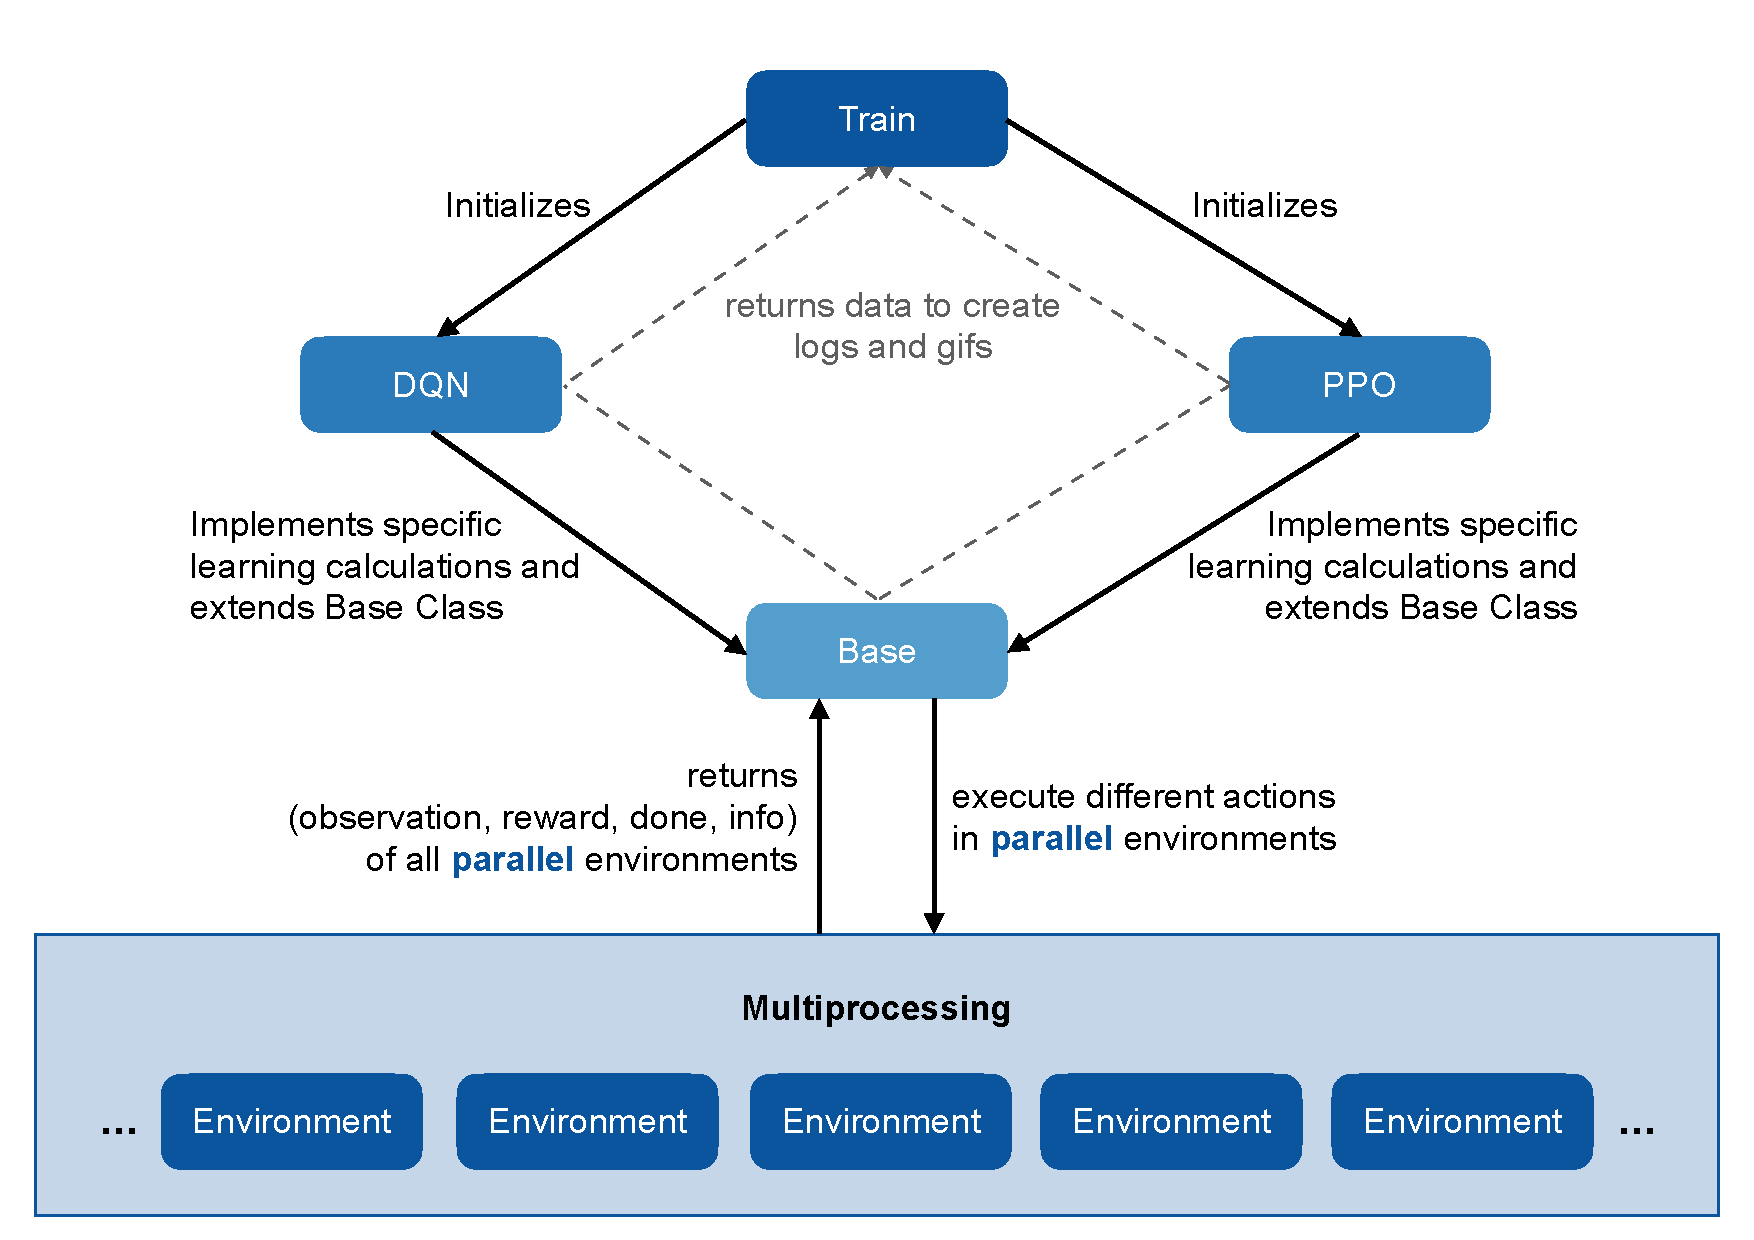
\includegraphics[width=0.9\textwidth]{pictures/training}\\
    \caption[The Training Structure]{The training structure}\label{fig:training}
\end{figure}

\marginpar{training setup}
First, the training of agents begins by generating n environments based on the \verb|--procs| setting of the training command, see Appendix \ref{ax:training_params} for the parameter list. Each environment has the same configurations, for example \verb|--grid-size|, \verb|--agents| and \verb|--agent-view-size|. Second, the amount of \verb|--frames| is taken from the parameters, defining a loop until that number is reached. In this case frames are equivalent to agent steps. During the loop, the defined training algorithm \verb|--algo| is executed.

\marginpar{base class}
Since both algorithms have similar procedures, they share the base class. In it experiences are gathered through a certain amount of actions which are executed on parallel environments. The action amount is set with \verb|--frames-per-procs|. During that period details like gained rewards, observations, actions and more are stored in base class variables that are accessible by the learning algorithms. When all experience actions are executed, the base variables are reset and log values are returned, as shown in Figure \ref{fig:training}. Afterwards the frame counter in the training script is updated with the amount of \verb|--frames-per-procs|. The training loop ends when the frames counter is greater or equal \verb|--frames|. Otherwise, more experience batches are gathered.

\marginpar{action selection}
Both learning algorithms include their own action selection methods. The PPO implementation relies on an actor-critic neural network, with an action space containing a probability distribution. In case of the DQN implementation the target network assigns Q values to actions, and agents choose one based on the maximum value with an epsilon greedy probability. In both variants the action selection results in one action for each agent and for each environment.

\subsection{DQN}
\marginpar{replay memory}
Unlike the PPO algorithm, in the DQN approach a quadruple of information is saved each frame into a replay memory. The four parts of the quadruple consist of the executed actions during that time step, the returned rewards and both the previous and new observation of the parallel environments. Until the frame amount of \verb|--initial-target-update| is reached, DQN agents only gather the quadruples but do not use them yet.

\marginpar{target update}
After exceeding the \verb|--initial-target-update|, the DQN learning starts. Each frame a batch of size \verb|--batch-size| is selected by randomly picking entries from the replay memory. Then, this batch is used to apply Q-learning updates to the experience samples, enhancing the training network. Every \verb|--target-update| amount of frames this training network is copied into the target network to enhance the action selection while keeping the algorithm stable.

The action selection itself is also improved during the training, by decreasing the $\epsilon$ gradually through $\epsilon = \epsilon_{end}+(\epsilon_{start}-\epsilon_{end})*e^{-\frac{frames}{decay}}$. This ensures exploration in the early phase. A high $\epsilon$ leads to actions that are picked at random. In the later course as the amount of frames increase, the $\epsilon$ gets smaller. In this case, the chance to select actions based on their Q values rises, which exploits the gathered experiences. Through \verb|--epsilon-start| and \verb|--epsilon-end| min and max values are set, and \verb|--epsilon-decay| defines the speed of reduction.

\subsection{PPO}
\marginpar{fill and reshape experiences}
In the DQN implementation learning happens during the base class batch creation, whereas in the PPO algorithm the learning process is triggered after the creation of each base class experience batch. The gathered values are reshaped and saved into a PPO experience buffer. Additionally, the advantage values are calculated here and added to the buffer.

\marginpar{optimize model}
With that experience buffer the PPO model is now optimized. A small number of \verb|--epochs| are iterated and during each iteration random batch entries are selected. With those entries the entropies, values and losses are calculated. Afterwards, the calculation results are used to update the policy and network, as suggested in the code of \ref{fig:ppo_algo_code}.

\section{Market Settings}\label{market_settings}
\marginpar{initialization}
To include a market into the training process, the \verb|--market| parameter can be set accordingly. The user has a choice to include an AM through the string ``am'' or a SM with ``sm''. In either case, the environment needs to adjust the action space, since agents have the option to conduct market transactions.

\marginpar{action space}
Per default, the environment action space is discrete and only contains five elements: moving up, down, left, right or wait. Adding a market expands that discrete space into a multi discrete space. Hence, both markets require actions in form of arrays that contain three elements. However, they use different information in the action array slots. This and further distinctions and detailed procedures of each market are explained separately in the following.

\subsection{Shareholder Market}
\marginpar{sm - action space}
A coloring environment that includes a SM constrains the first position of the action array to one of the five environment actions. The next position contains an agent index, towards which a buying offer will be made. Although, if this number is higher than the amount of agents in the game, the action intends no buying transaction. The last array position contains either a zero or a one, with one signalizing that the agent wants to sell its share. An abstract representation of a shareholder action array is: \verb|[environment_action, agent_index, sell_share]|.

\begin{figure}[hpbt]
    \centering
    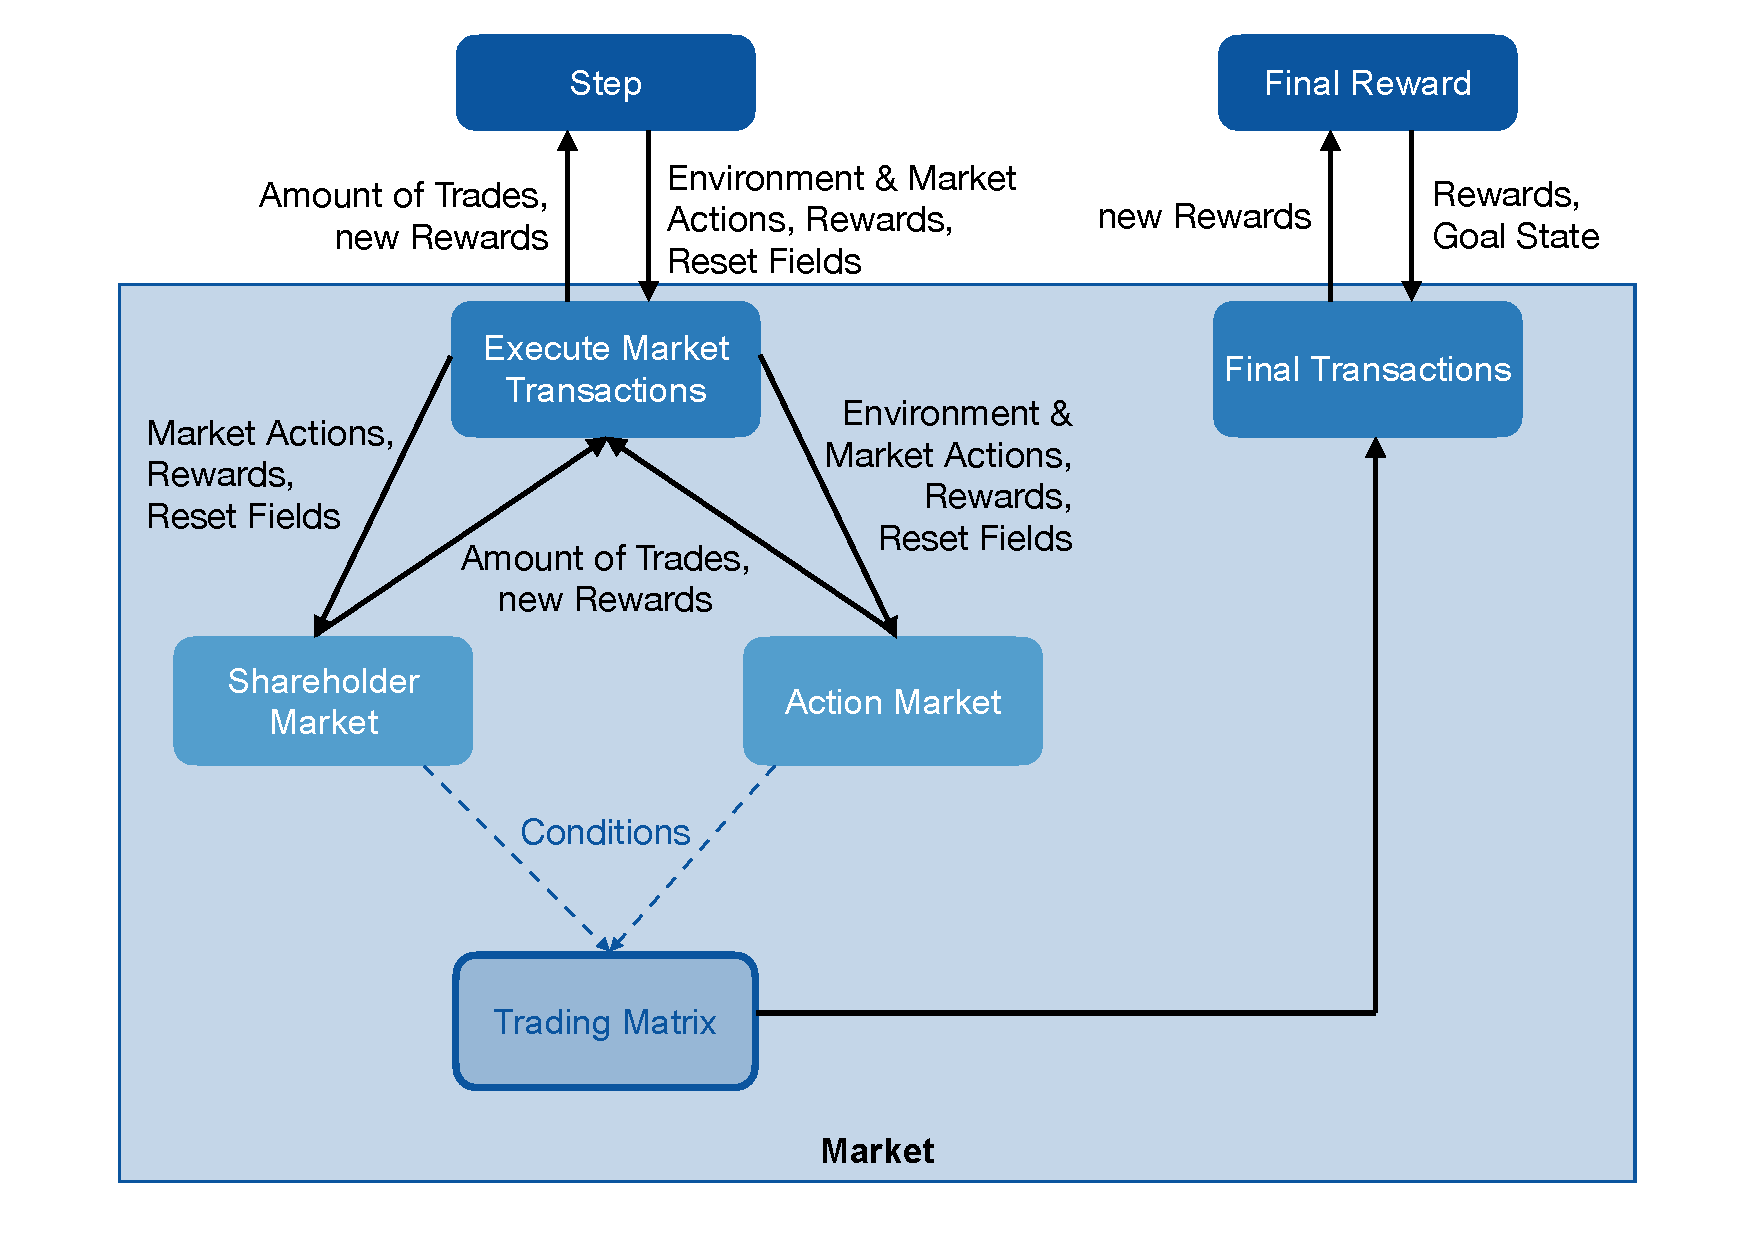
\includegraphics[width=0.9\textwidth]{pictures/market}\\
    \caption[Market Elements]{The market elements}\label{fig:market}
\end{figure}

\marginpar{shareholder market step}
In Figure \ref{fig:market} market elements are visualized. On the left, the process that takes place during each step is shown, see algorithm \ref{algo:step_reward} line 10. Here, the market always receives an action array that is already divided in two parts, one part only containing the first array position and the other the buying and selling information in this case.
% Since transactions alter the rewards, the current reward is also transmitted. Lastly, an array of agent indices that have recently reset cells is also given, since some transaction conditions make use of that information.

\marginpar{trading matrix}
In the course of the market calculations a trading matrix is altered. This matrix is quadratic with dimensions equal to the amount of agents. In a shareholder trading matrix, the diagonal contains ones, since every agent starts with the full ownership over their own shares. All other matrix slots are filled with zeros. An example for an initial trading matrix is shown below.
\begin{equation*}
trading\_matrix = 
\begin{pmatrix}
1 & 0 \\
0 & 1
\end{pmatrix}
\end{equation*}

\marginpar{market transactions - matrices}
The first thing to check in a market step execution is the market type. If the SM matches, the corresponding function is called. 
% In this case the environment actions are not of importance, so the function receives all other parameters instead. 
Inside the shareholder function two additional matrices are created from the market actions, a buying matrix and a selling matrix. Both matrices are initially filled with zeros, are quadratic, and their dimensions depend on the amount of agents, similar to the trading matrix. The buying matrix contains a one in the row of the buyer and the column of the agent that the offer is directed to.
% Here, the diagonal stays zero, since agents are prohibited of buying from themselves. 
Each agent can only buy one share at a time, therefore the rows contain at maximum one entry. The selling matrix may contain ones only on the diagonal and only for the agent that wants to sell according to the market actions.

\marginpar{iteration}
After setting up the two matrices they are iterated, extracting buyer, seller and the corresponding matrix rows. A transaction takes place if the following conditions are met:
\begin{itemize}
    \item the buyer is not equal to the seller
    \item all entries of the buyer row and the seller row match
    \item the sellers shares are greater than the \verb|--trading-fee|
\end{itemize}

\marginpar{transaction}
If all conditions are true, the trading matrix is updated here, by changing the share of the selling agent, adding the subtracted amount to the buyer. The amount can be set with \verb|--trading-fee|, which is 0.1 per default. The last condition ensures, that agents still receive some of their own rewards and do not trade everything off. 

\marginpar{example}
An example for a transaction could be two agents acting in an environment. If agent 2 buys a share from agent 1, the trading matrix is updated. The second row stores the shares of agent two, which increase by 0.1 on the first position. This signalizes that agent 2 is owner of some shares of agent 1 and still has 100\% of its own shares. In response, the shares in the first row and column of agent 1 decreases to 0.9.
\begin{equation*}
trading\_matrix = 
\begin{pmatrix}
1 & 0 \\
0 & 1
\end{pmatrix} \xrightarrow[\text{from Agent 1}]{\text{Agent 2 buys}} 
trading\_matrix = 
\begin{pmatrix}
0.9 & 0 \\
0.1 & 1
\end{pmatrix} 
\end{equation*}

\marginpar{rewards}
Additionally, the rewards of the current step calculation, would be updated here, if a price for the shares are set. In this implementation however, the shares have no price since agents are willing to give them away for free. Otherwise, the price would be subtracted from the buying agents' reward and that value would be added to the reward of the selling agent. Nonetheless, in this implementation the SM triggers a reward redistribution according to the trading matrix in each step. 

The details of this calculation will be discussed in \ref{market_reward_calc}.
Lastly, the transaction count is documented for evaluation purposes. At this point the market execution is done and the number of executed trades and the updated rewards are returned.

\subsection{Action Market}
\marginpar{action space}
The agent action shape of an AM environment is similar to the shareholder action array. Again, an action has three slots, with the first being the environment execution and the second being the index of an agent a buying offer will be directed to. The difference to a shareholder action is the last array position. Instead of setting a bit here to signalize the willingness of selling shares, the agent chooses an environment action that is expected from the agent of position two. Hence, an abstract representation of an action in the AM is the following: \verb|[environment_action, agent_index, expected_action]|.

\marginpar{transaction}
The market elements and general process of visualization \ref{fig:market} also apply to an AM setting. Here however, the trading matrix is initially filled with zeros. 
% Furthermore, the AM function needs all parameters, including the environment actions. This information is crucial to the transaction conditions, which are:
To establish a transaction in this market setting the following conditions must be met:
\begin{itemize}
    \item the buyer differs from the receiving agent
    \item the environment action of the receiving agent matches the expected action
\end{itemize}

\marginpar{success}
When the two conditions apply a market transaction takes place. The \verb|--trading-fee| parameter decides the price the buyer pays the receiving agent. Both the rewards and trading matrix are altered here, by subtracting the price from the buyer and adding it to the receiver. An example of the trading matrix update in this market setup is shown below. Here again Agent 2 is purchasing from Agent one.
\begin{equation*}
trading\_matrix = 
\begin{pmatrix}
0 & 0 \\
0 & 0
\end{pmatrix} \xrightarrow[\text{from Agent 1}]{\text{Agent 2 buys}} 
trading\_matrix = 
\begin{pmatrix}
0 & 0.1 \\
0 & -0.1
\end{pmatrix} 
\end{equation*}

The trading matrix stores the market balance of both agents in each row. For agent 2 this means that the negative value was spent. The first row shows that agent 1 still has a neutral balance and gained the \verb|--trading-fee| of 0.1 from agent 2. To conclude, the market returns the number of transactions that took place in this step and the new rewards.

\subsection{Reward Calculations}\label{market_reward_calc}
\marginpar{intro}
During each step agents can update the trading matrix by acting on the market. With each update the rewards are also changed. In Figure \ref{fig:market_rewards} a detailed example of the reward update in a market is shown. It is worth mentioning that it is not possible to execute both markets simultaneously, but rather one or none must be set for a training process. This illustration shows both calculations in one image for convenience. Equal to the previous examples, the red agent 2 buys a share or action from the blue agent 1. For both market scenarios the \verb|--trading-fee| is set to the default value and both agent rewards start at 0.1. On the top half of the image the internal market calculation of a SM is shown, and the bottom half illustrates the calculation of an AM.
\begin{figure}[hpbt]
    \centering
    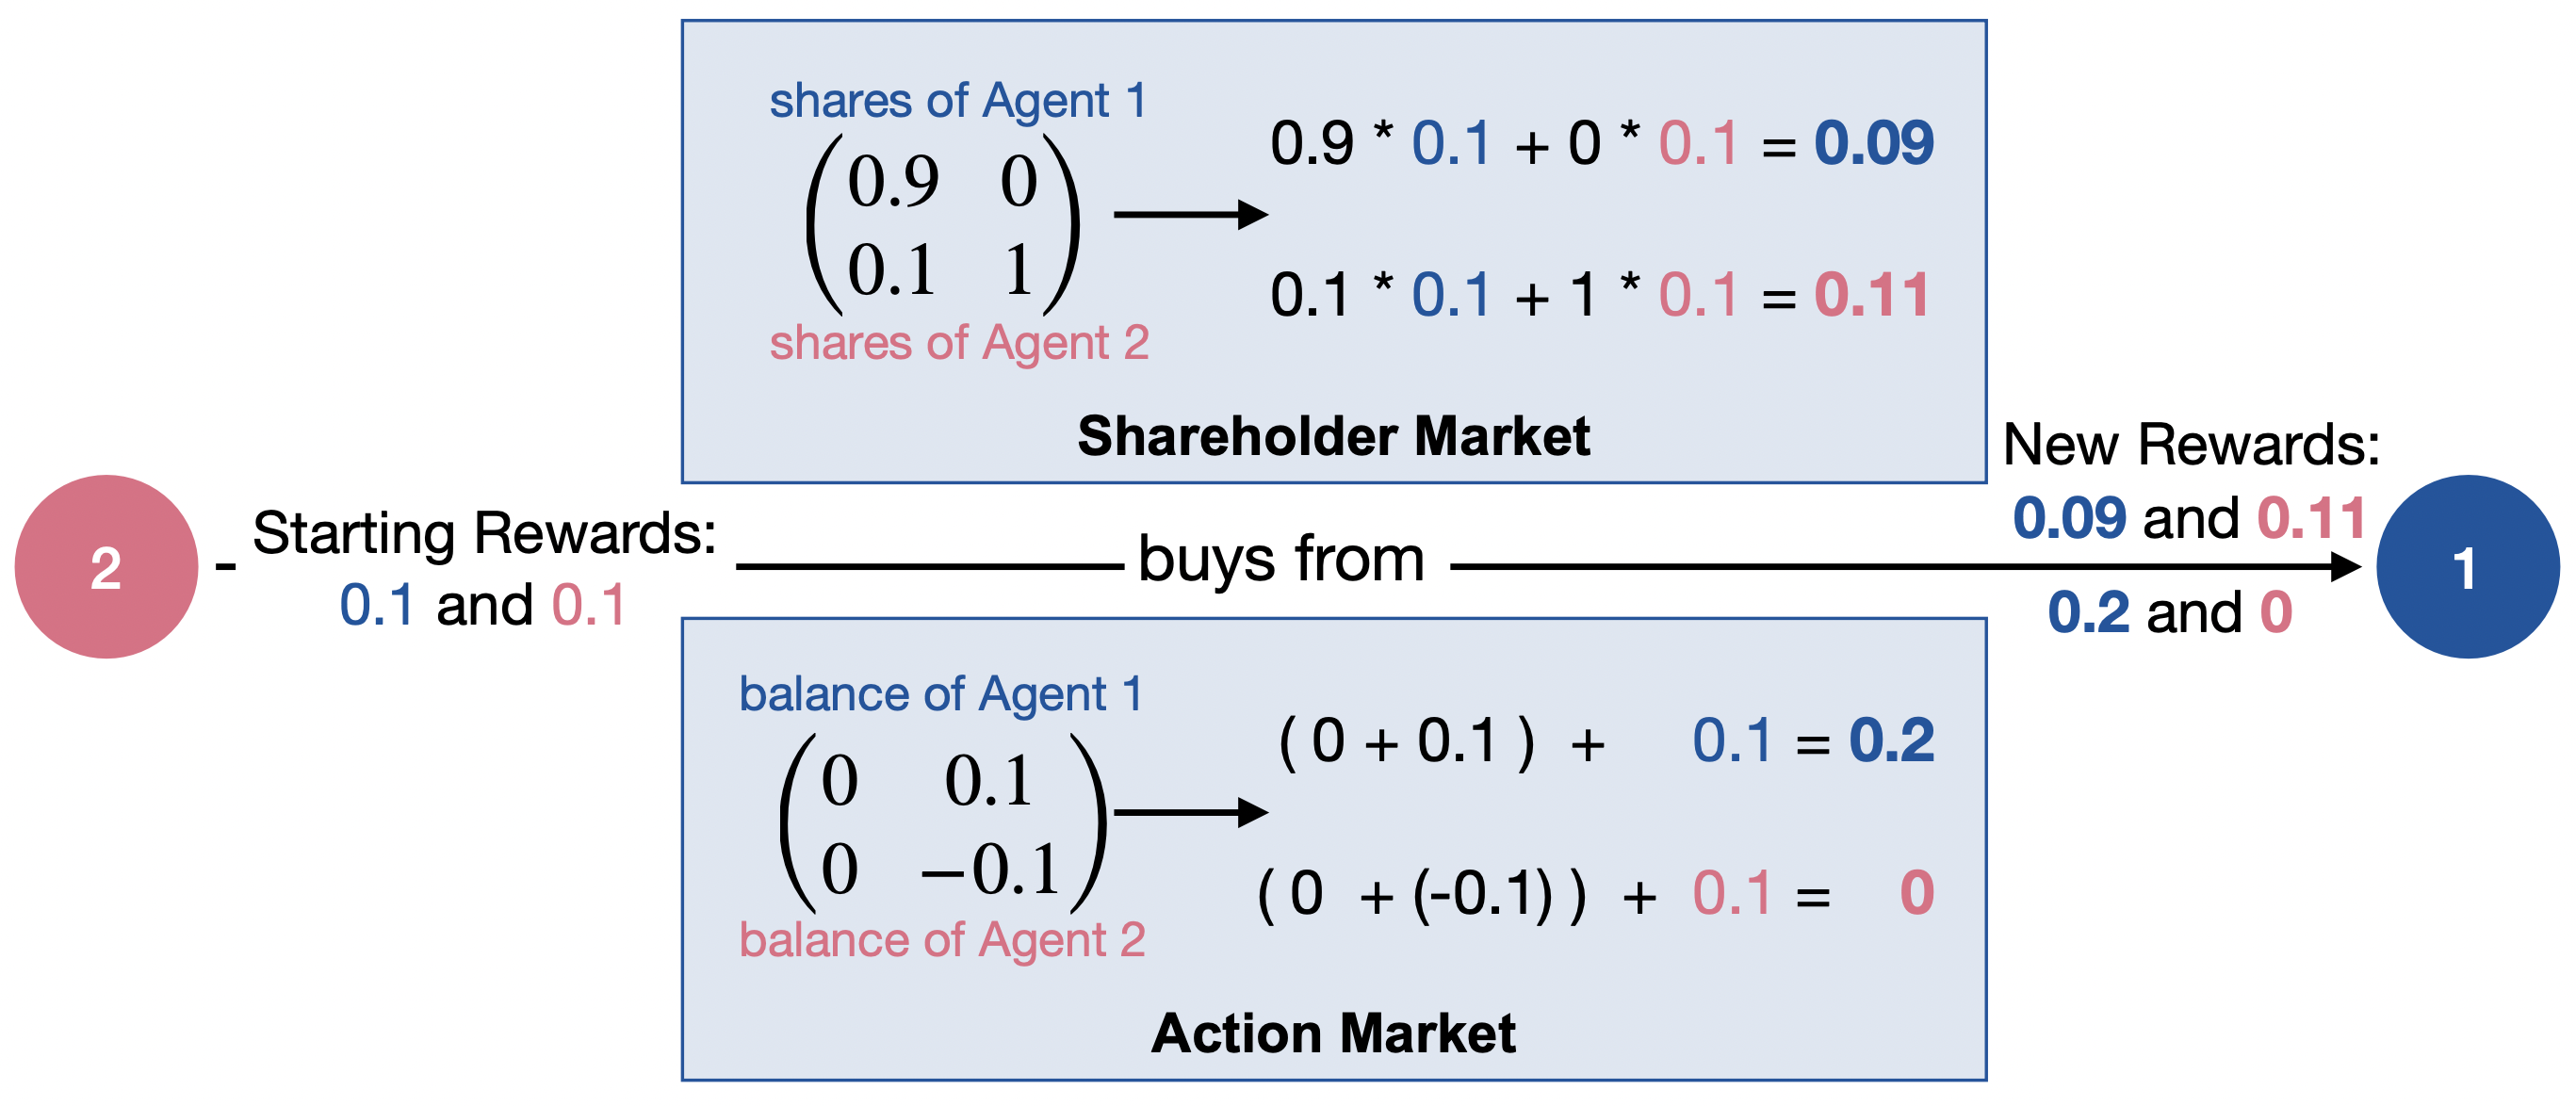
\includegraphics[width=0.9\textwidth]{pictures/new_market_rewards}\\
    \caption[Exemplary Reward Calculation Of Markets]{Exemplary reward calculations of both market types}\label{fig:market_rewards}
\end{figure}

\marginpar{sm matrix}
In a SM the trading matrix represents the distribution of agent shares. Each matrix column adds up to one, representing a 100\% share of an agent. As mentioned earlier the diagonal of the matrix is initially set to 1 since agents start with complete ownership over their shares. For this example the trading matrices are configured accordingly. The first matrix row implies that Agent 1 is owner of 90\% of its own shares and is not owner of any shares from agent 2. Whereas the second row shows that agent 2 claims 10\% of the shares of agent 1 and has full ownership over its own.

\marginpar{sm calculations}
To generate the new rewards of the agents, the market multiplies all current rewards with each matrix rows. The resulting products of each row are then summed up to represent the new reward of the corresponding agent. For the example, agent 1 gets a new reward value of 0.09 and Agent 2 claims 0.01 from agent 1 and adds that to its full value of 0.1, resulting in a new reward of 0.11. 

\marginpar{sm calculations}
In contrast to an AM in a SM the rewards are just reassigned based on the current shares of the trading matrix. An exception occurs, when agents have negative rewards. In this case their share will be skipped during the redistribution, since shares are used to participate in profits. 

\marginpar{sm calculations}
Another difference to AMs is that the shown SM reward redistributions are executed in each step, and it is irrelevant whether market action were executed. The only exception however is the last step, when the done flag is set to true. In this case the final rewards, see algorithm \ref{algo:final_reward}, need to be calculated first, before the shares are taken into account.

\marginpar{am calculations}
AMs, in most cases, update the rewards directly and only once, when a transaction is executed. The trading fee is immediately subtracted from one agents' reward and added to the counterpart during the trade. If an agent can not afford the fee the process is completed anyway and the agent goes into debt. 

\marginpar{am trading matrix}
Thus, this market type makes no use of the trading matrix. Nonetheless, the matrix is always updated, since a specific scenario requires the calculations to be executed at the end, see section \ref{market_conditions}. In this case, the agents market balance, stored in the matrix rows, is summed up and added to the current reward. This procedure is illustrated in the bottom half of figure \ref{market_reward_calc}. Here, the fee of 0.1 is subtracted from agent 2 and added to the reward of agent 1, leading to new rewards of 0.2 for agent 1 and zero for agent 2.

\subsection{Additional Conditions}\label{market_conditions}
\marginpar{reset}
The \verb|--market| string for both types can be extended to add more conditions, namely with ``no-reset'', ``no-debt'' and ``goal''. The ``no-reset'' string enables the check whether the buyer has recently reset a cell. If that is the case, the corresponding buyers are ignored on the market for the current step. Hence, their market actions will not be applied. However, in a SM the penalized agent can still sell its shares. 

\marginpar{debt}
With the ``no-debt'' Flag, transactions only take place if buyers can afford to pay the price. In this implementation with AMs and the default fee, this is solely the case if agents have colored a cell in that step. Waiting or misbehaving agents are excluded as buyers, since their rewards result in 0 or -0.1. For SMs this depends on the presence of a share price. Per default the price is zero, similar to the approach of Schmid et al. \cite{scbe21}, making this condition irrelevant for the SM setting.
% TODO kommt zu goal Both market conditions can be used simultaneously.

\marginpar{goal}
The last addition, ``goal'', lets the market process run as usual, only removing the reward changes during the steps. Here, all transactions are just documented into the trading matrix during an episode. Eventually, the transactions are executed once the final rewards of algorithm \ref{algo:final_reward} is calculated. As shown on the right side of Figure \ref{fig:market}, the market obtains those rewards and a Boolean describing whether the environment goal was reached.

\marginpar{conditions}
The rewards are updated with the trading matrix content when either of the two conditions is satisfied:
\begin{itemize}
    \item ``goal'' addition is present and environment goal was reached
    \item no ``goal'' addition and market type is a SM
\end{itemize}
Otherwise the rewards are return as they are and will not be processed further. 

For such goal oriented markets, regardless of the type, the final environment state needs to equal the overall aim. Thus, the whole grid has to be colored, to execute the final market transactions.

% Since the goods of a SM are shares, naturally the current reward values are of importance. During the step calculations of the rewards the done flag is  takes place at the end of an episode. In an AM however, each step is self-contained in regards to transactions and payouts. Nonetheless, with the ``goal'' addition, the payout also shifts to the end of episodes. 

\marginpar{trading matrix}
If the first condition applies and an AM is present the rewards are updated by using the trading matrix. For a SM either condition must be met in order to generate the final reward. The calculations for both cases are equal to the example of chapter \ref{market_reward_calc}.
% Again, the trading matrix rows and rewards are iterated here. Each row element is multiplied with the reward of the same index and added to the new reward of that agent. An example of both operations is shown in Figure \ref{fig:market_rewards}.

\marginpar{returns}
After the final market updates to the rewards the new values are returned, as shown in Figure \ref{fig:market}. The last thing to point out is that the additional market conditions can be used in combination, making ``sm-goal-no-reset-no-debt'' for example a valid \verb|--market| setting.

